

\documentclass{article}

\usepackage{pgfplots}
\pgfplotsset{width=7cm,compat=1.8}
\usepackage{graphicx}
\usepackage{hyperref}
\usepackage{tikz}
\usepackage{pgfplots}
\usepackage[romanian]{babel}


\author{Eduard-Mihail Hamza}
\title{Evoluția reliefului fitness}

\begin{document}
\maketitle

\section{Introducere}
În analiza matematică, un punct de maximum reprezintă cea mai mare valoare pe care o poate lua funcția fie pe un anumit interval, caz în care se numește maxim local, sau pe întreg domeniul de definiție, caz în care se numește maxim global.\\
Bazinul de atracție al unui punct de maxim local se definește ca mulțimea de puncte inițiale pentru care căutarea ne duce spre același optim.\\
În acest raport se va prezenta evoluția reliefului fitness atunci când se utilizază algoritmul de Hill Climbing cu variantele First Improvment și Best Improvment, specificându-se în acest sens punctele de maxim local și bazinele lor de atracție.

\section{Metode}
Pentru găsirea maximului global al funcției se va folosi metoda
\textbf{Hill Climbing}, o metodă iterativă ce realizează o căutare locală. Este utilizată varianta iterată (Iterated Hill Climbing) în care HC este restartat, pentru a mări gradul de explorare a spațiului de căutare.\\
De asemenea, se vor folosii 2 tipuri de HC:  \textbf{Best Improvment Hill Climbing} și \textbf{First Improvment Hill Climbing}\\
\textbf{Best Improvment Hill Climbing} examinează fiecare vecin și îl alege pe cel care determină cea mai bună soluție.\\
\textbf{First Improvment Hill Climbing} nu examinează fiecare vecin înainte de a hotărî pe care îl alege. Pur și simplu alege un vecin la întâmplare pâna când gasește unul mai promițător decât cel curent.\\



\section{Experiment}
Experimentul se va realiza pe următoarea funcție:

$$ f(x) = x^{3} - 60 \cdot x^{2} + 900 \cdot x + 100, x \in [0, 31]$$
Maxim pe intervalul [0, 31]: 4100 (x = 10).

\begin{figure}[!h]
  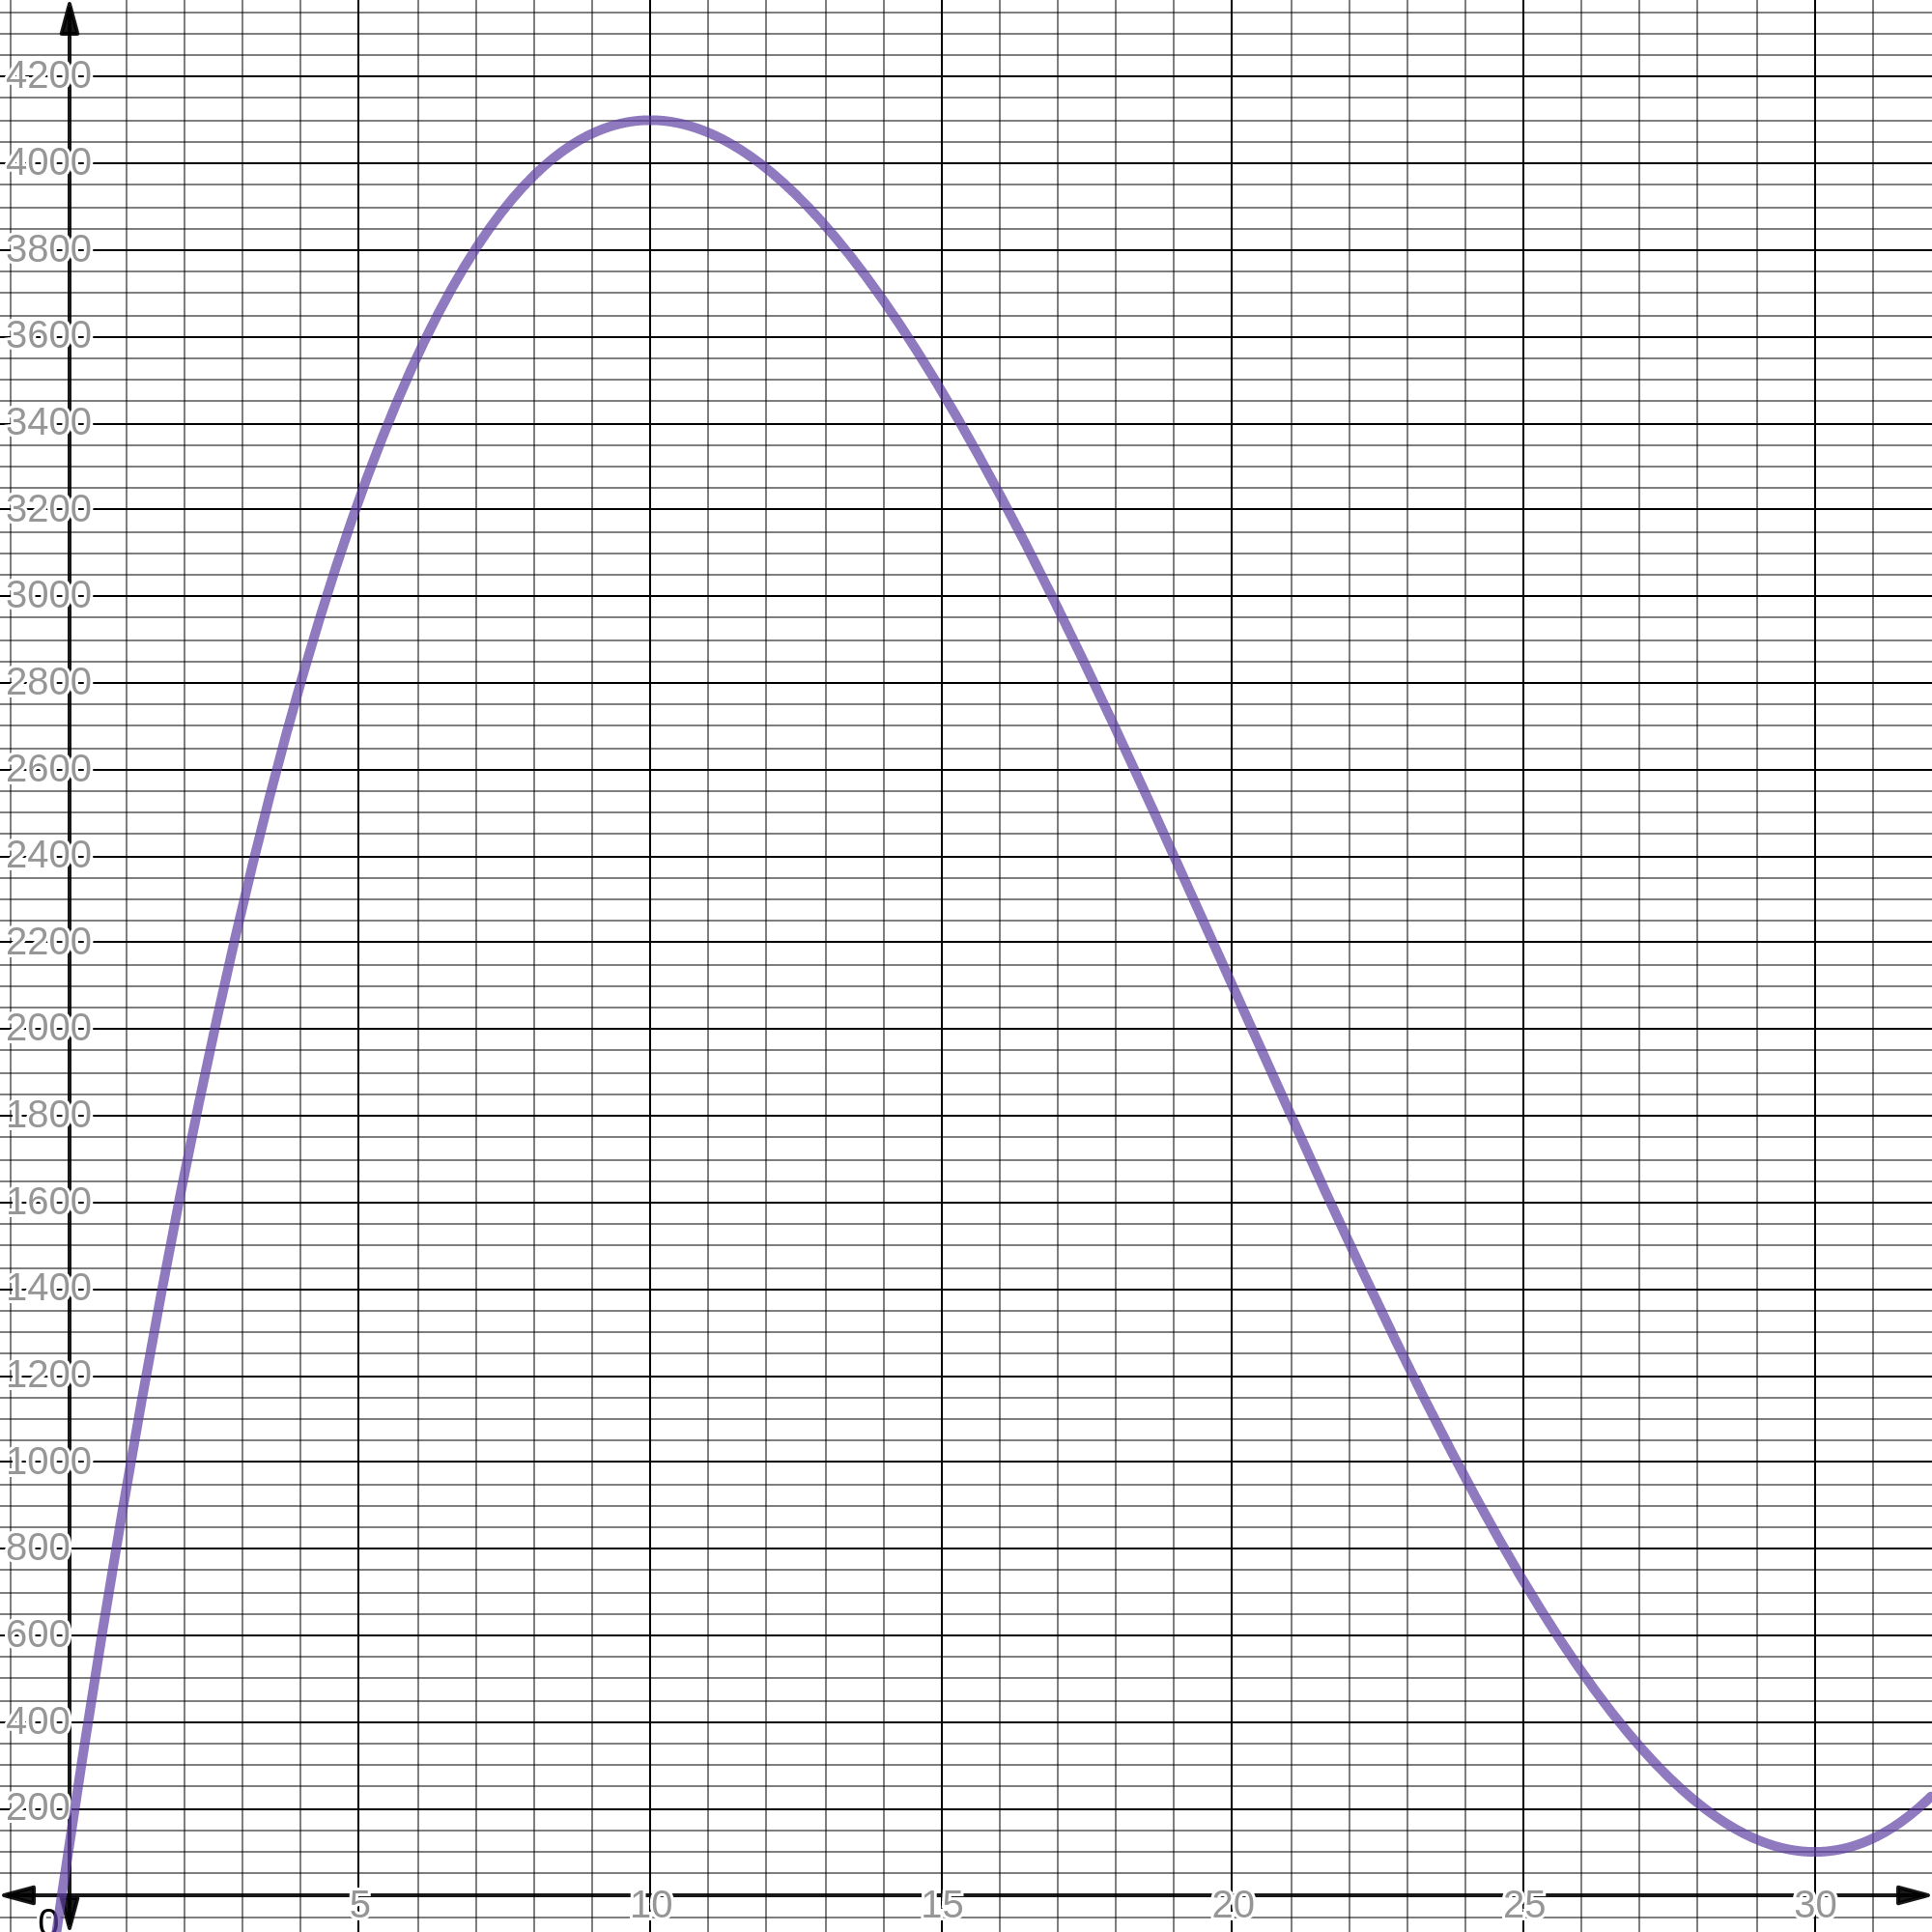
\includegraphics[width=\textwidth,height=\textheight,keepaspectratio]{desmos-graph.png}
  \caption{Graficul funcției de test}
\end{figure}

\section{Results}
\subsection{First Improvment}

\begin{figure}[!h]
\begin{tabular}{||c|||l||}
  \hline
  Maxim local & Bazin de atracție \\ \hline \hline
  7 & 0, 1, 2, 3, 4, 5, 6, 7, 15, 20, 21, 22, 23, 28, 29, 30, 31\\ \hline
  10 & 0, 1, 2, 3, 4, 5, 6, 8, 9, 10, 11, 13, 14, 15, 20, 21, 22, 23, 24, 25, 26, 27, 28, 29, 30, 31 \\ \hline
  12 & 0, 1, 2, 4, 5, 6, 8, 12, 13, 14, 15, 20, 21, 22, 23, 24, 25, 26, 27, 28, 29, 30, 31\\ \hline
  16 & 0, 1, 2, 3, 16, 17, 18, 19, 20, 21, 22, 23, 24, 25, 26, 27, 28, 29, 30, 31 \\ \hline
\end{tabular}
\caption{Bazin de atracție First Improvment - monstră statistică 30}
\end{figure}

\subsection{Best Improvment}

\begin{figure}[!h]
\begin{tabular}{||c|||l||}
  \hline
  Maxim local & Bazin de atracție \\ \hline \hline
  7 & 23, 7, 6, 22 \\ \hline  
  10 & 0, 1, 2, 3, 5, 8, 9, 10, 11, 13, 14, 15, 21, 24, 25, 26, 27, 29, 30, 31 \\ \hline
  12 & 12, 28, 4\\ \hline
  16 & 16, 17, 18, 19, 20 \\ \hline
 
\end{tabular}
\caption{Bazin de atracție Best Improvment - monstră statistică 30}
\end{figure}



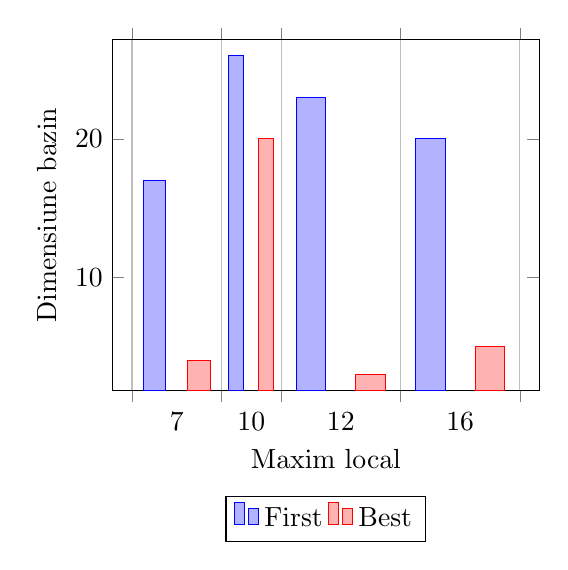
\begin{tikzpicture}
\begin{axis}[
	x tick label style={
		/pgf/number format/1000 sep=},
	ylabel=Dimensiune bazin,
	xlabel=Maxim local,
	enlargelimits=0.05,
	legend style={at={(0.5,-0.3)},
	anchor=north,legend columns=-1},
	ybar interval=0.5,
]
\addplot 
	coordinates {(7, 17) (10, 26)
		 (12, 23) (16, 20) (20, 20)};
\addplot 
	coordinates {(7, 4) (10, 20)
		 (12, 3) (16, 5) (20, 20)};
\legend{First, Best}
\end{axis}
\end{tikzpicture}



\subsection{Interpretare}
Atât varianta Best Improvment, cât și varianta First Improvment returnează aceleași maxime locale \textbf{7, 10, 12, 16}.\\ 
\textbf{Varianta First Improvment} are o dimensiune a bazinelor foarte mare pentru toate maximele locale, iar multe numere se regăsesc în bazinul mai multor maxime. De exemplu numerele 0, 1, 2, 30, 31 se găsesc in bazinele tuturor celor 4 maxime locale.\\
\textbf{Varianta Best Improvment} are o dimensiune a bazinelor mult mai redusă. De asemenea, fiecare număr din intervalul [0, 31] se regăsește într-un singur bazin de atracție.\\
Se observă că punctul în care se atinge maximul global (x=10) este și punctul cu bazinul de atracție cel mai mare, atât pentru Fisrt Improvment cât și pentru Best Improvment.

\section{Concluzie}
În concluzie, ambele metode produc aceleași maxime locale. Diferența dintre First Improvment și Best Improvment este că primul are bazine de atracție de dimensiune mult mai mare decât al doilea, iar în ceea ce priveste unicitatea numerelor, Best Improvment are doar numere diferite pentru fiecare bazin, în vreme ce First Improvment are multe numere ce se află in bazinele de atracție a mai multor maxime locale.



\begin{thebibliography}{9}

\bibitem{wikipedia}
  Maximum și minimum\\
  \url{https://en.wikipedia.org/wiki/Maxima_and_minima}
  
\bibitem{Overleaf}
  Bar Graph\\
  \url{https://www.overleaf.com/learn/latex/pgfplots_package}

\bibitem{Grafic funcție}
  Grafic funcție\\
  \url{https://www.desmos.com/calculator}
  
\bibitem{Site curs}
  Site curs și laborator\\
  \url{https://profs.info.uaic.ro/~eugennc/teaching/ga/}
  
\bibitem{Site curs}
  Tipuri de Hill Climbing\\
  \url{https://www.geeksforgeeks.org/introduction-hill-climbing-artificial-intelligence/}

\end{thebibliography}  
\end{document}
